\documentclass{beamer}
\usepackage{beamerthemesplit} % kam neu dazu
\usepackage[utf8]{inputenc}
\usepackage[T1]{fontenc}
\usepackage[ngerman]{babel}



\begin{document}
\title{Mößbauereffekt} 
\author{Paul Kremser, Tobias Grussenemyer}
\date{Versuchsdurchführung: 1. bis 12. März 2010} 

\frame{\titlepage} 

\frame{\frametitle{Inhaltsverzeichnis}\tableofcontents} 

\section{Einleitung}
\subsection{Historisches}
\subsection{Anwendungen}

\frame{\frametitle{Rudolf Mößbauer}
Er ging davon aus, dass sich zwei Quanten die auf diese Weise wechselwirken mit der doppelten Rückstoßgeschwindigkeit aufeinander zu bewegen müssten.
Diese Theorie folgt direkt aus der Impulserhaltung und schien zunächst auch durch das Experiment bestätigt zu werden. Zuerst untersuchte Mössbauer nämlich die
Resonanzabsorption bei Zimmertemperatur und darüber. Als er aber begann Quelle und Absorber abzukühlen, stieg die Intensität des Messsignals plötzlich steil an,
und zwar über die bei hohen Temperaturen gemessene.
}

\section{Theorie und Aufbau}
\subsection{Emission und Absorption}

\frame{\frametitle{Emission und Absorption}
\begin{columns}
\column{.55\textwidth}
\begin{enumerate}
 \item \textcolor{blue}{Emission}: In der Quelle zerfällt angeregter Zustand (Skizze) und erzeugt Gammastrahlung
 \item \textcolor{blue}{Absorbtion}: Gammastrahlung regt Kern im Absorber an, Kern wird kurz angeregt
 \item \textcolor{blue}{Resonanzabsorbtion}: Quelle und Absorber gleichen Materials
\end{enumerate}
\column{.45\textwidth}
\centering 
\begin{figure}[H]  
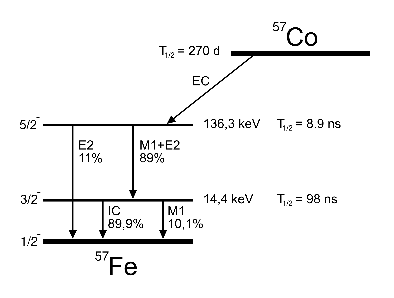
\includegraphics[width=0.95\linewidth]{pictures/zerfall_quelle.eps}
\end{figure}
\end{columns}
\vfill
Bei beiden Vorgängen wird Energie übertragen $\Rightarrow$ Linien verschoben
}

\frame{\frametitle{Energieübertrag}
\begin{columns}
\column{.55\textwidth}
\begin{itemize}
 \item \textcolor{blue}{Emission}:\\
Rückstoßimpuls $p_R = -p_{\gamma}$\\
Energieübertrag $E_R = \frac{p_{\gamma}^2}{2m} = \frac{E_{\gamma}^2}{2mc^2}$\\
Quant verliert Energie $\Rightarrow E_{\gamma} = E_0-E_R$ 
 \item \textcolor{blue}{Absorbtion}:\\
Rückstoßimpuls $p_R = p_{\gamma}$\\
Quant kann nur absorbiert werden wenn $E_{\gamma} = E_0+E_R$
\end{itemize}
\column{.45\textwidth}
\centering 
\begin{figure}[H]  
\includegraphics[width=0.95\linewidth]{pictures/linienskizze1.ps}
\end{figure}
\end{columns}
\vfill
Linien sind um $2E_R$ gegeneinander verschoben, also ist keine Resonanzabsorption möglich
}

\frame{\frametitle{Linienbreite}
Die Breite der Energielinien ist durch zwei Effekte gegeben
\begin{itemize}
 \item \textcolor{blue}{natürliche Linienbreite $\Gamma$}: \\
  resultiert aus Energie-Zeit-Unschärfe, diese verknüpft $\Gamma$ mit mittlerer Lebensdauer $\tau$\\
 \begin{align*}
  \tau \Gamma = \hbar \Rightarrow \Gamma = \frac{\hbar}{\tau}
 \end{align*}
 \item \textcolor{blue}{Dopplerverbreiterung}: \\
  resultiert aus Bewegung der Atome, durch Dopplereffekt wird Frequenz $\nu_0$ verschoben:
 \begin{align*}
  \nu = \nu_0 * \left( 1 + \frac{v}{c} \right)
 \end{align*}
\end{itemize}
}
\subsection{Rückstoßfreie Resonanzabsorbtion}

\frame{\frametitle{Kerne im Gitter}
Wenn Kerne in Gitter gebunden sind wird der Rückstoßimpuls auf das Gitter übertragen
\begin{itemize}
\item in Imbulsbilanz erhöht sich die Masse der Kerne auf Gittermasse 
\item fast kein Energieübertrag auf den Kern bei Emission 
\item Absorbtion kann stattfinden, da auch hier kaum Energieübertrag
\end{itemize}
\vfill
$\Rightarrow$ Resonanzabsorbtion möglich
}

\frame{\frametitle{Kerne im Gitter}
\includegraphics[width=0.95\linewidth]{pictures/linienskizze.ps}
}

\frame{\frametitle{Anregung von Gitterschwingungen}
Im Gitter können allerdings Gitterschwingungen angeregt werden
\begin{itemize}
 \item tritt auf, wenn Rückstoßenergie Phonon erzeugen kann
 \item Gammaquant fehlt Energie $\Rightarrow$ keine Resonanzabsorption
\end{itemize}
\vfill
$\Rightarrow$ Debye-Waller-Faktor gibt Anteil elastisch gestreuter Photonen an
}

\frame{\frametitle{Debye-Waller-Faktor}
Debye-Waller-Faktor $f$ ist Verhältniss von elastischer Streuung und Absorbtion durch Gitterschwingungen.
\begin{align*}
 f = exp\left[ -\frac{3E_R}{2k_B\Theta}\left(1+\left(\frac{2T}{\Theta}\right)^2 \int\limits_{0}^{\frac{\Theta}{T}} \frac{x~dx}{e^x - 1}\right)\right]
\end{align*}
für kleine Temperaturen $(T<<\Theta)$ und Kerne im arteigenen kubischen Gitter:
\begin{align*}
 f \approx exp \left[ -\frac{E_R}{k_B\Theta}\left(\frac{3}{2} + \left(\frac{\pi T}{\Theta}\right)^2\right)\right]
\end{align*}
$\Theta$ ist die Debye-Temperatur, eine Materialkonstante.
\vfill
$\Rightarrow f$ sollte möglichst groß sein
}

\frame{\frametitle{Temperaturabhängigkeit Debye-Waller-Faktor}
\centering 
\begin{figure}[H]  
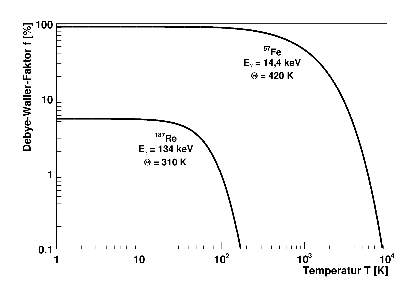
\includegraphics[width=0.75\linewidth]{pictures/debye.eps}
\end{figure}
}

\frame{\frametitle{Temperaturabhängigkeit Debye-Waller-Faktor}
\centering 
\begin{figure}[H]  
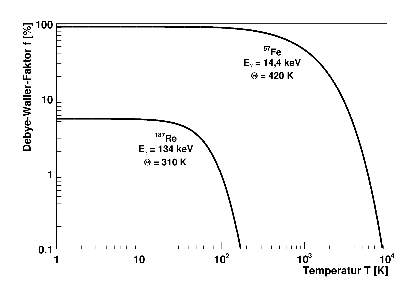
\includegraphics[width=0.75\linewidth]{pictures/debye.eps}
\end{figure}
\hfill
Für $^{57}Fe$ Debye-Waller-Faktor bei Raumtemperatur > 90\% \\
}
\subsection{Hyperfeinstruktur und Isomerieverschiebung}


\frame{\frametitle{Hyperfeinstruktur}
\begin{columns}
\column{.55\textwidth}
\begin{itemize}
 \item Entartung des Kernspins wird durch Magnetfeld $B$ aufgehoben, neue Wechselwirkungsenergie $E_{mag}$
\begin{align*}
 E_{mag}=\frac{\mu_l m_l}{l}B
\end{align*}
 \item Zustände spalten in $2l+1$ Unterniveaus auf
 \item Auswahlregel $\Delta m_l = 0, \pm 1$ \\
$\Rightarrow$ sechs mögliche Übergänge \\
\end{itemize}
\column{.45\textwidth}
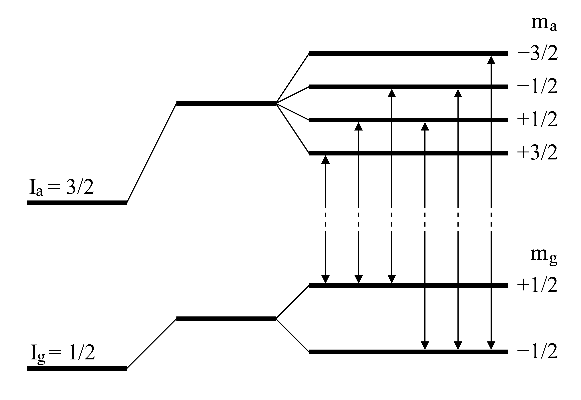
\includegraphics[width=0.9\linewidth]{pictures/termshema_eisen.eps}
\end{columns}
\vfill
$\Rightarrow$ Transmissionskurve ist 6-Linien Spektrum
}

\frame{\frametitle{Isomerieverschiebung}
Durch unterschiedliche Materialien in Absorber und Quelle verursacht
\begin{columns}
\column{.55\textwidth}
\begin{itemize}
 \item unterschiedliche La\-dungs\-dich\-te\-ver\-teil\-ung\-en von Kern im Grundzustand und angeregtem Kern
 \item Elektronen\-hülle erzeugt unterschiedliche Coulomb\-energien
\end{itemize}
\column{.45\textwidth}
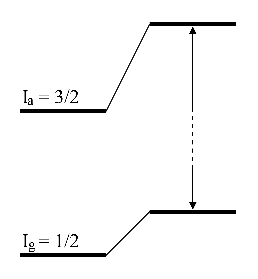
\includegraphics[width=0.9\linewidth]{pictures/isomerie.eps}
\end{columns}
\vfill
$\Rightarrow$ Möglichkeit der Analyse chemischer Bindungen
}
\subsection{Aufbau}
\frame{\frametitle{Frequenzdurchstimmung mittels Dopplereffekt}
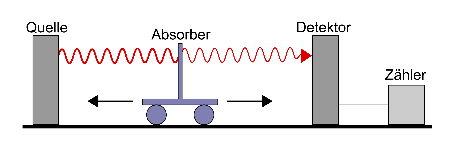
\includegraphics[width=0.9\linewidth]{pictures/aufbau_doppler.eps} \\
Absorber wird mit konstanter Geschwindigkeit $v$ bewegt \\
\vfill
$\Rightarrow$ Dopplerverschiebung der Übergangsfrequenz $\nu_0$ zu
 \begin{align*}
  \nu(v) = \nu_0 * \left( 1 + \frac{v}{c} \right)
 \end{align*}
}

\frame{\frametitle{Versuchsaufbau mit Elektronik}
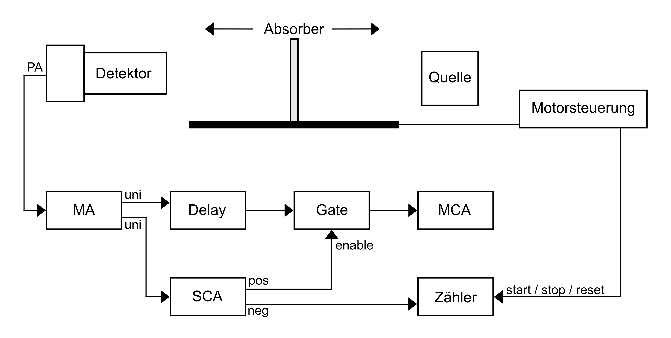
\includegraphics[width=0.9\linewidth]{pictures/aufbau_el.eps} \\
Elektronik soll Impulse des Detektors filtern \\
\vfill
$\Rightarrow$ nur relevante Impulse des Detektors werden gezählt
}

\section{Durchführung und Ergebnisse}
\subsection{Aufgabenstellung}
\frame{\frametitle{Aufgabenstellung}
\begin{enumerate}
 \item Energieeichung des MCA
 \item Energiefenster auf 14,4 KeV Linie
 \item Untergrundmessung
 \item Spektrum des 1-Linien- (Eisen) Absorbers
 \begin{itemize}
  \item Isomerieverschiebung
  \item Effektive Absorberdicke, Wirkungsquerschnitt, Debye-Waller-Faktor
  \item Linienbreite und Lebensdauer
 \end{itemize}
 \item Spektrum des 6-Linien- (Edelstahl) Absorbers.
 \begin{itemize}
  \item Isomerieverschiebung
  \item Kernmagnetisches Moment
  \item Magnetfeld am Kernort
 \end{itemize}
\end{enumerate}
}

\subsection{Energieeichug und Energiefenster}
\frame{\frametitle{Energieeichung}
\begin{block}{Wofür Energieeichung}
 Zur Identifikation des 14,4$keV$ Peaks im Spektrum \\
 $\Rightarrow$ Beziehung zwischen Kanal des MCA und Energie 
\end{block}
\begin{block}{Wie}
 Americium-Quelle mit verschiedenen Metallplättchen \\
 $\Rightarrow$ Bekannte Energien mit identifizierbaren Peaks
\end{block}
\vfill
\begin{tabular}{|l|l|l|l|l|l|}
\hline
Stoff & Rubidium & Molibdän & Silber & Terbium & Barium\\
Energie $K_{\alpha}$/keV & 13.3 & 17.44 & 22.1 & 44.23 & 32.06 \\
\hline
\end{tabular}

}
\frame{\frametitle{Gaußfits an $K_\alpha$-Linien}
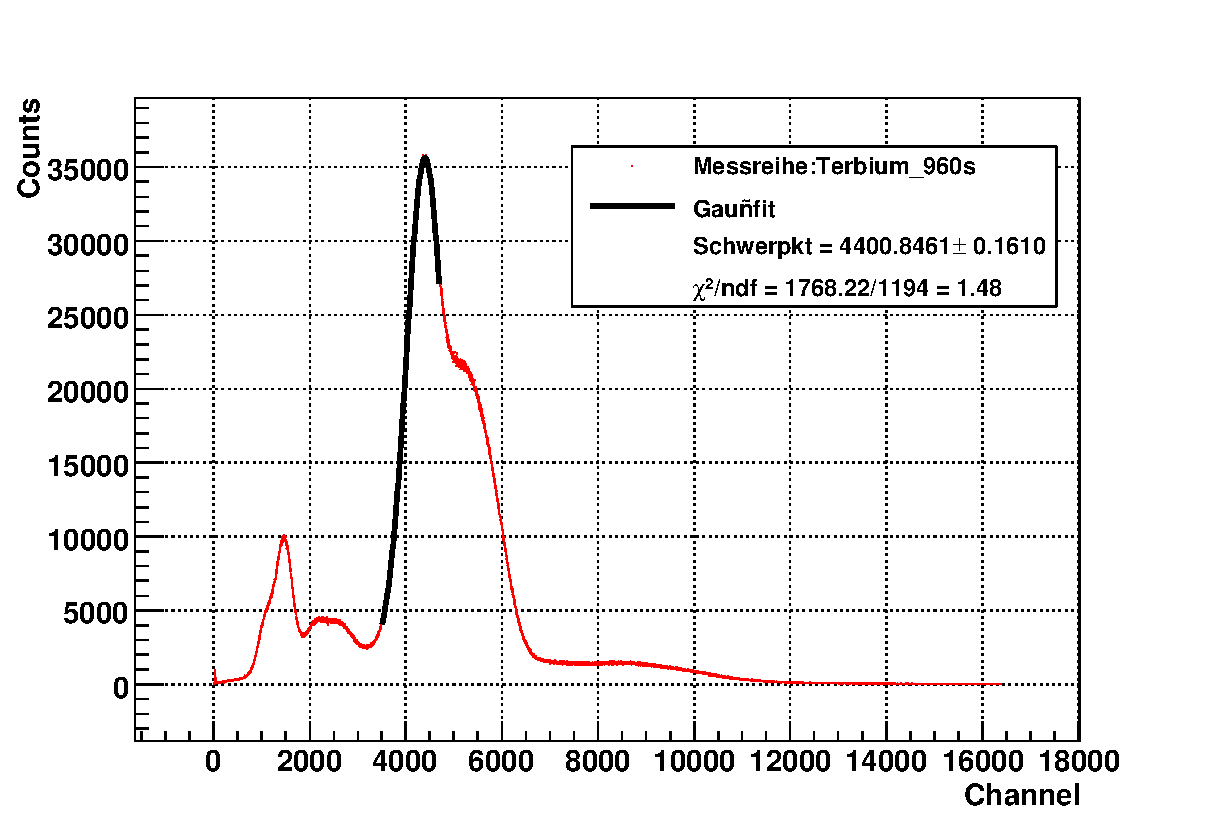
\includegraphics[width=0.9\linewidth]{pictures/eichung_terbium.eps}
}
\frame{\frametitle{Gaußfits an $K_\alpha$-Linien}
\begin{columns}
        \column{.5\textwidth}
                 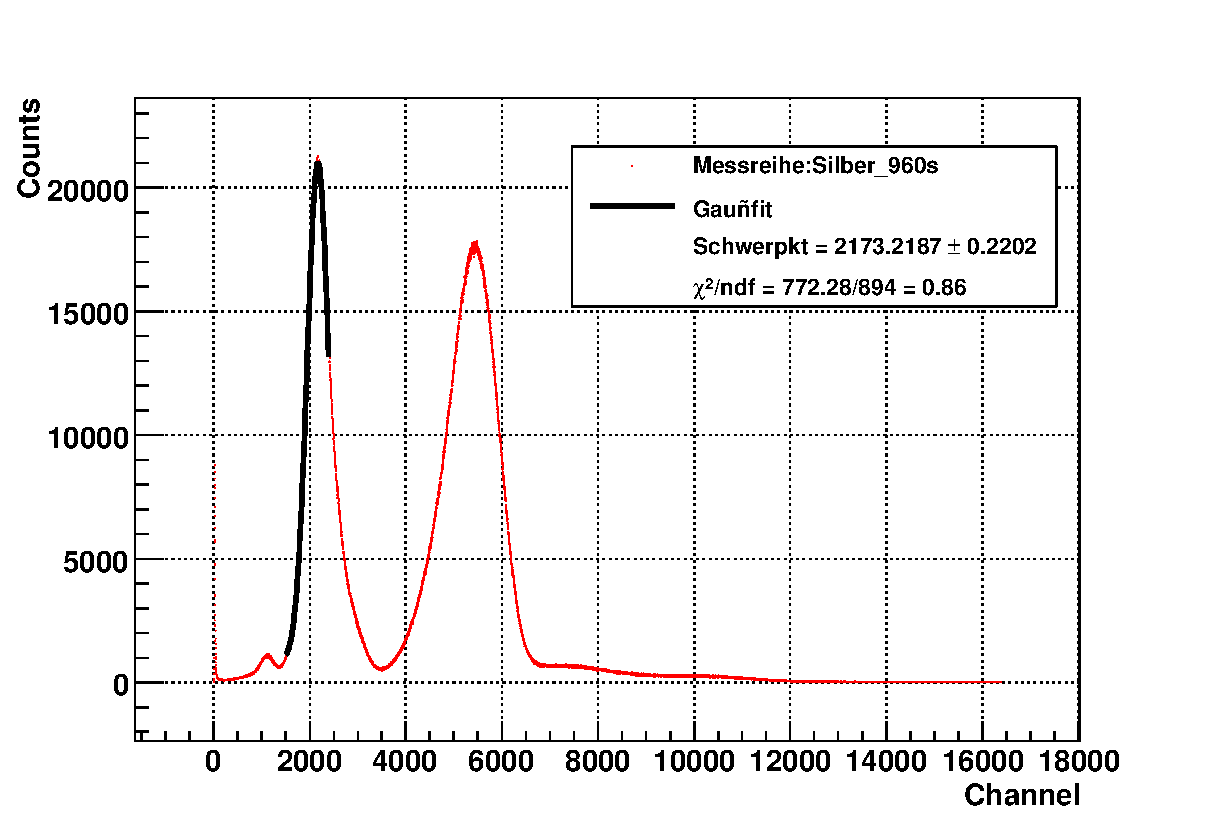
\includegraphics[width=0.9\linewidth]{pictures/eichung_silber.eps}
        \column{.5\textwidth}
		 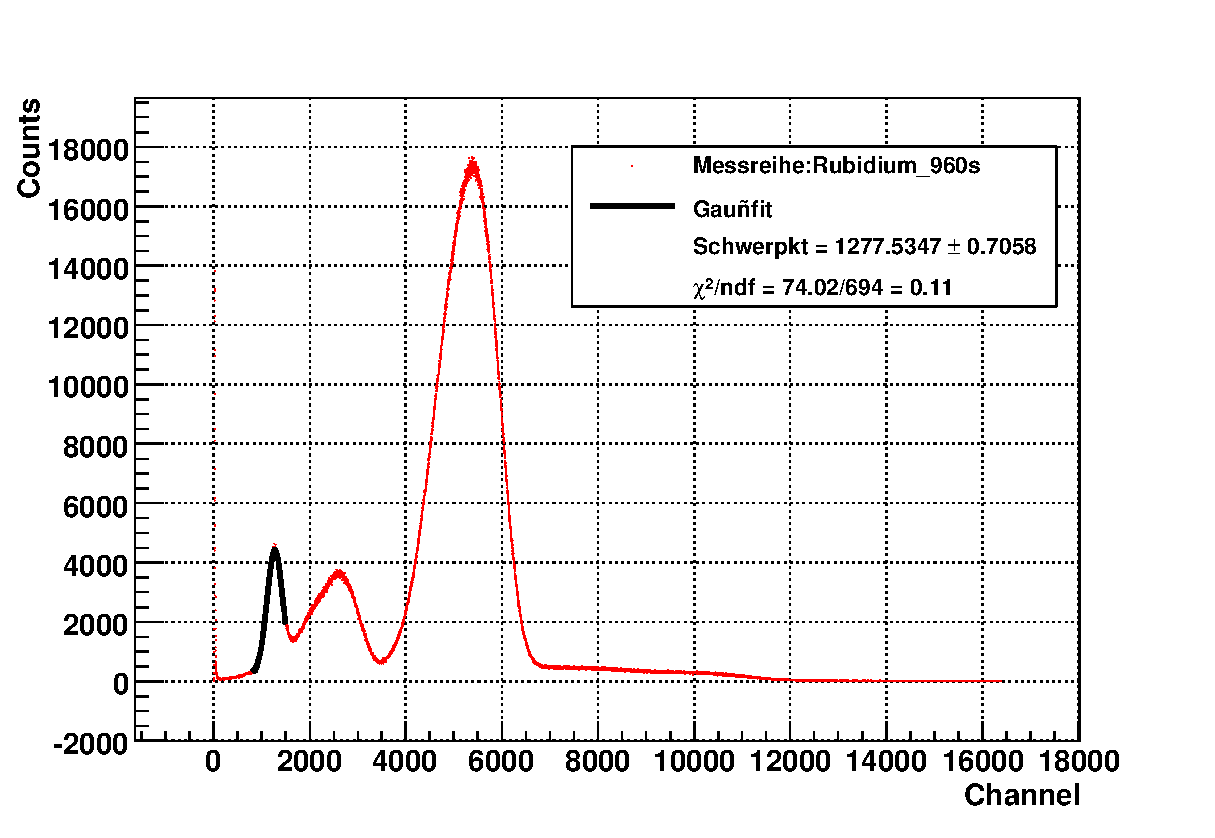
\includegraphics[width=0.9\linewidth]{pictures/eichung_rubidium.eps}
\end{columns}
\begin{columns}
        \column{.5\textwidth}
                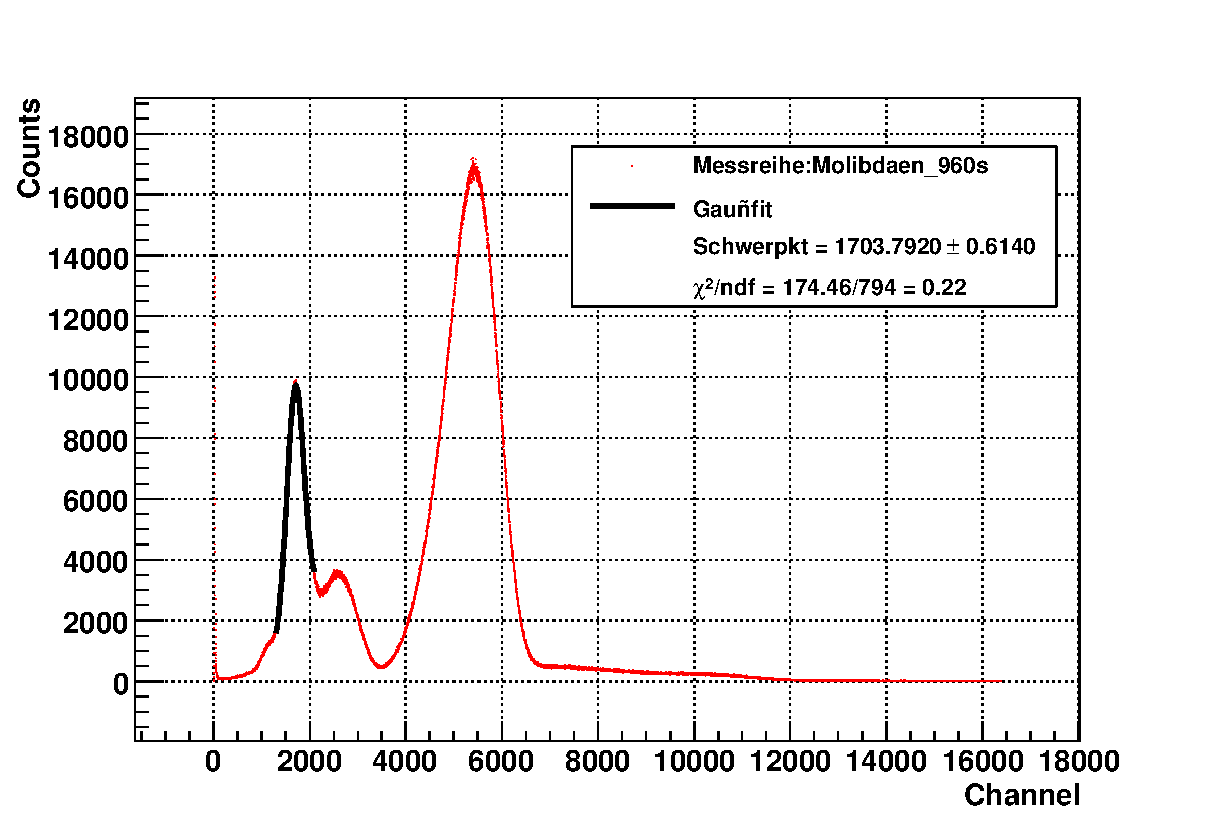
\includegraphics[width=0.9\linewidth]{pictures/eichung_molibdaen.eps}
        \column{.5\textwidth}
                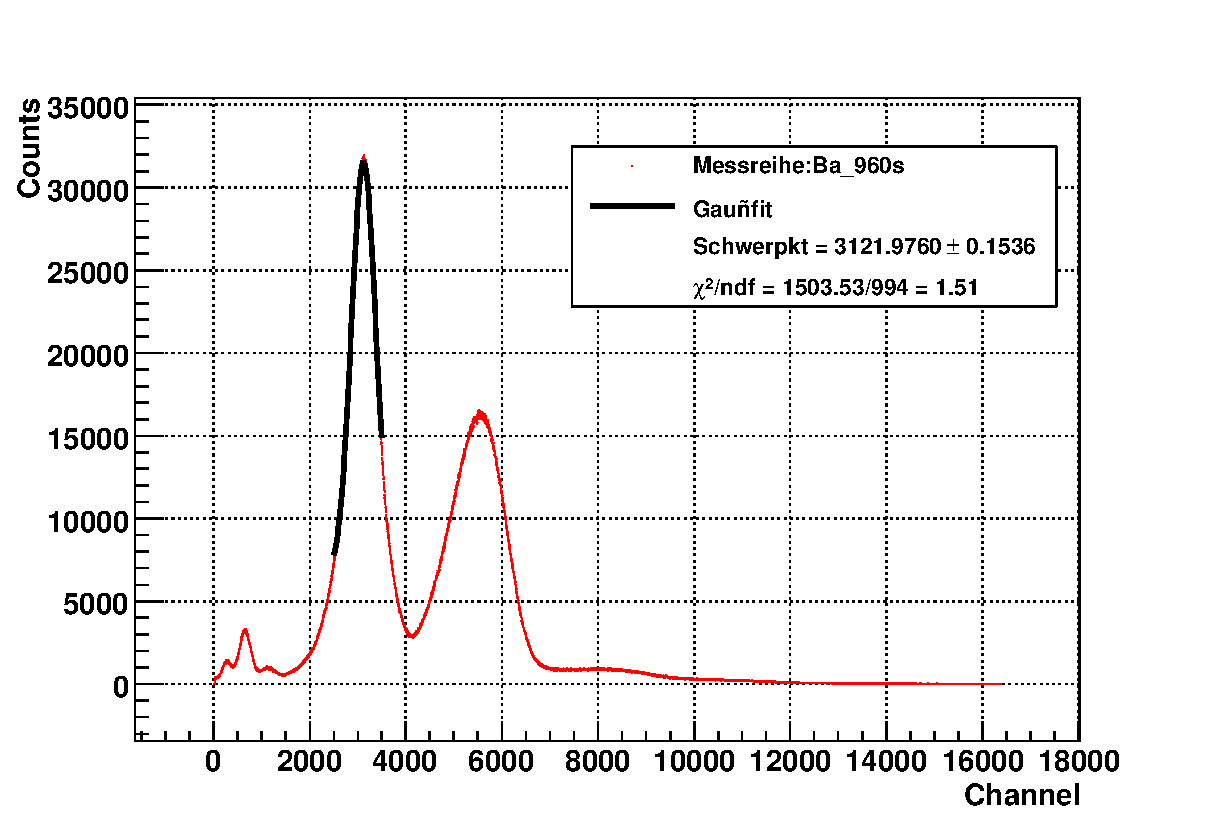
\includegraphics[width=0.9\linewidth]{pictures/eichung_barium.eps}
\end{columns}
}
\frame{\frametitle{Fit an die Orte der Gaußkurven}
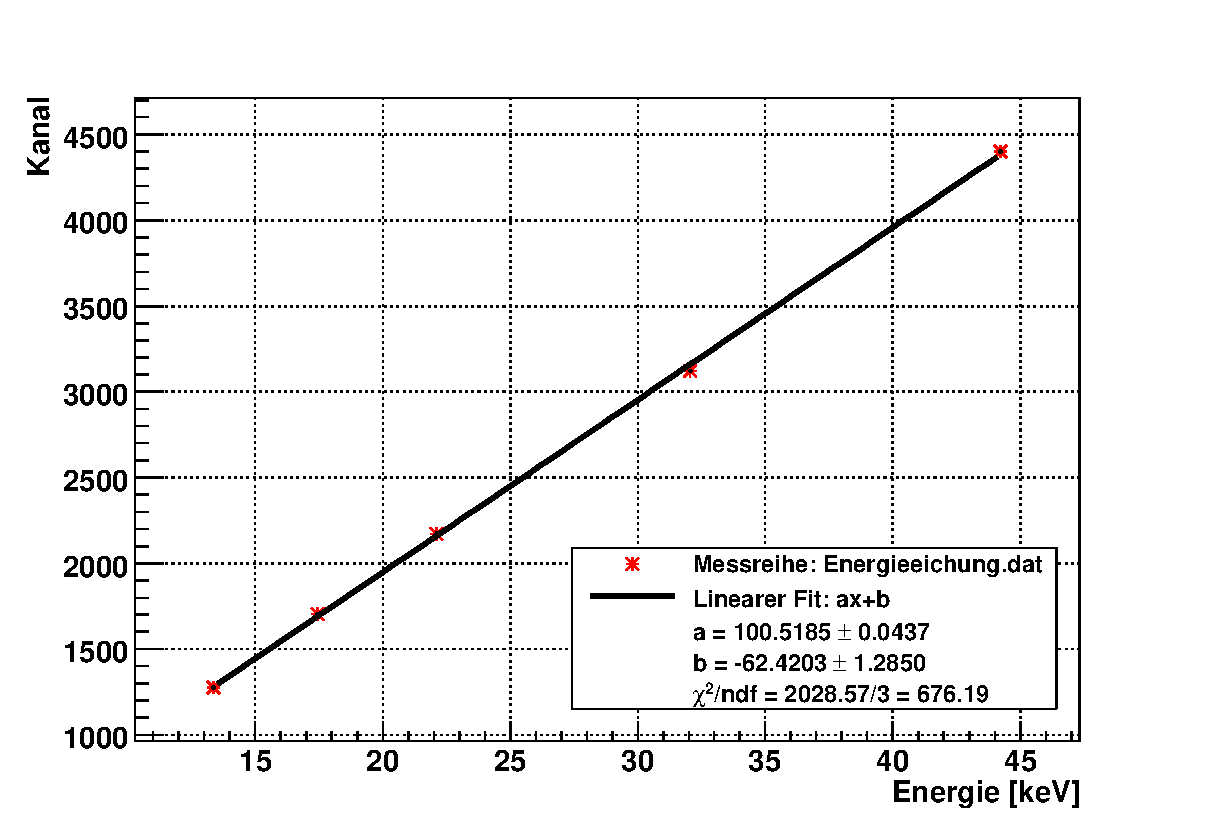
\includegraphics[width=0.9\linewidth]{pictures/eichung_linear.eps}
}
\frame{\frametitle{Fit an die Orte der Gaußkurven}
\begin{block}{Fit}
\begin{align*}
  C = a \cdot E + b \hspace{30pt}
\end{align*}
\begin{align*}
 \textnormal{mit}\hspace{30pt}a = 100.52 \pm 0.04\textnormal{ und }b =  -62.42 \pm 1.285
\end{align*}
\end{block}

\begin{block}{14,4 keV Linie}
\begin{align*}
  C_{14.4keV} = 1385,07 \pm 1,27
\end{align*}
\end{block}
}
\frame{\frametitle{Fenstereinstellung}
\begin{block}{Warum ein Fenster verwenden}
 Mößbauermessung geschieht mit Zähler, getriggert durch Motor \\
 $\Rightarrow$ Nur Ereignisse mit 14,4 keV sollen gezählt werden
\end{block}
\begin{block}{Single-Channel-Analyser}
 Einstellung: Unter- und Obergrenze für Energie \\
 Visualisierung über MCA
\end{block}
}
\subsection{Untergrund}
\frame{\frametitle{Untergrund}
\begin{block}{Compton-Streuung}
\begin{itemize}
 \item Quelle hat im wesentlichen zwei Peaks ($14,4 keV$ und $122 keV$)
 \item Comptonstreuung erzeugt Untergrund im Messfenster
 \item Nur indirekt messbar
\end{itemize}
\end{block}
\begin{block}{Abschirmung durch Aluminium}
Bei zunehmender Dicke erwartet man unterschiedliche Abschwächung der beiden Energien \\
$\Rightarrow$ Doppelter Expotentialfit und Extrapolation auf Dicke 0
\end{block}
}
\frame{\frametitle{Untergrundfit}
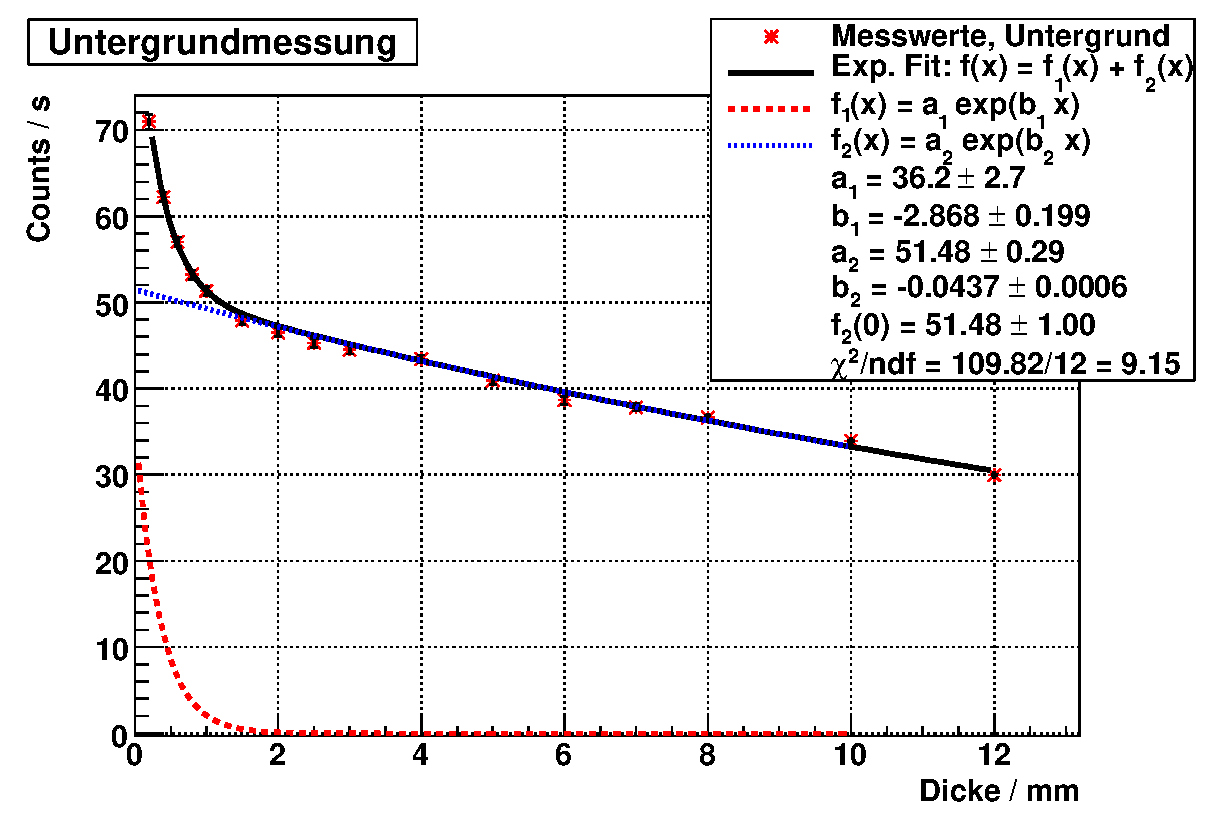
\includegraphics[width=0.9\linewidth]{pictures/untergrund.eps}
}
\frame{\frametitle{Untergrundfit}
\begin{block}{Fit}
\begin{align*}
  f_2 (d) = (50,38 \pm 0,78) \cdot exp (-0,0413 \pm 0,0027) \frac{Counts}{s}
\end{align*}
\end{block}

\begin{block}{Untergrundzählrate}
\begin{align*}
  R_{Untergrund} = (50,38 \pm 0,78) \frac{Counts}{s} 
\end{align*}
\end{block}
}
\subsection{Die Messung}
\frame{\frametitle{Absorberschlitten und Zähler}
\begin{block}{Absorberschlitten}
 Absorberschlitten wird über Getriebe mit Motor angetrieben
\begin{itemize}
 \item 2 Übersetzungen (20:1 und 5:1)
 \item Geschwindigkeiten von 0,01$\frac{mm}{s}$ bis 10$\frac{mm}{s}$
\end{itemize}
\end{block}

\begin{block}{Zähler}
 Der Zähler wird von der Motorsteuerung gesteuert
 $\Rightarrow$ Es wird nur gezählt wenn die Fahrgeschwindigkeit konstant ist
\end{block}
}
\frame{\frametitle{Absorberschlitten und Motor}
%\includegraphics[width=0.9\linewidth]{pictures/motor.eps}
}
% 1 Linien (Edelstahl)
\frame{\frametitle{Edelstahl-(1-Linien-)absorber}
\begin{block}{Der Absorber}
 Edelstahl, unmagnetisch, 25$\mu m$ Dick
\end{block}
\begin{block}{Absorberbewegung}
\begin{itemize}
 \item Geschwindigkeiten von $-2,5\frac{mm}{s}$ bis $2,5\frac{mm}{s}$ \\
 $\Rightarrow$ Dopplerverschiebung von $\pm 1,2 \cdot 10^{-7} eV$ 
 \item Geschwindigkeitsvariation $\Rightarrow$ Verschiebung Absorptions- gegen Emissionslinie
\end{itemize}
\end{block}
}
\frame{\frametitle{Spektrum}
\begin{block}{Transmissionsprofil}
\begin{itemize}
 \item Transmissionsprofil näherungsweise Lorentzförmig
 \item Abweichung da dicker Absorber verwendet
 \item Lorentzfit zu schmal
\end{itemize}
\end{block}

\begin{block}{Voigt-Fit}
 \begin{itemize}
  \item Faltung von Lorentz und Gauß
  \item Lorentzanteil liefert direkt die natürliche Linienbreite
 \end{itemize}
\end{block}
}
\frame{\frametitle{Lorentz-, Gauß- und Voigt-Fit}
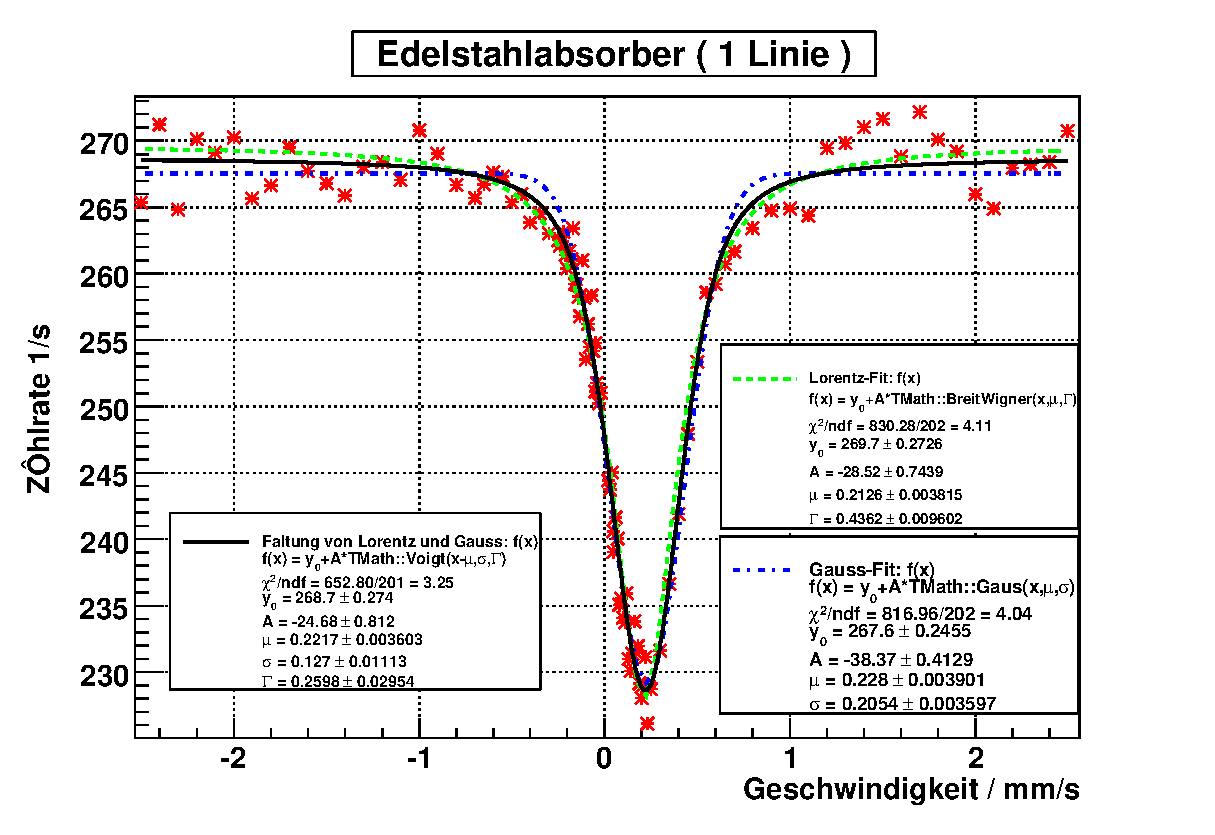
\includegraphics[width=0.9\linewidth]{pictures/edelstahl.eps}
}
\frame{\frametitle{Isomerieverschiebung}
\begin{block}{Isomerieverschiebung}
 Die Isomerieverschiebung lässt sich aus der Lage des Transmissionsminimum direkt ablesen \\
 Wir erhielten:
\begin{align*}
 v_{iso} = (0.22\pm 0.0026) \frac{mm}{s}
\end{align*}
Umgerechnet in Energie:
\begin{align*}
 E_{iso} = (10.7 \pm 0.12) 10^{-9} eV
\end{align*}
\end{block}
}
\frame{\frametitle{Linienbreite}
\begin{block}{Linenbreite aus Voigt-Fit}
 Aus dem Lorentzanteil des Voigt-Fits ergibt sich eine Linenbreite von:
\begin{align*}
 \Gamma = ( 7 \pm 0,53) \cdot 10^{-9} eV
\end{align*}
Der Literaturwert beträgt:
\begin{align*}
 \Gamma = 4,64 \cdot 10^{-9} 
\end{align*}
\end{block}
}
\frame{\frametitle{Linienbreite}
\begin{block}{Linenbreite alternativ}
\begin{itemize}
 \item Bestimmung der relativen Verbreiterung aus der effektiven Absorberdicke
 \item Berechnung der natürlichen Linenbreite aus Lorent-Fit
\end{itemize}
Damit ergibt sich:
\begin{align*}
 \Gamma = (5.09 \pm 0.14) 10^{-9} eV
\end{align*}
\end{block}
\vfill
Abweichung: Ungenaue Angaben über Absorber, Quelldicke unbekannt
}
% 6 Linien (Eisen)
\frame{\frametitle{Eisen-(6-Linien-)absorber}
\begin{block}{Der Absorber}
 Natureisen, ferromagnetisch
\end{block}
\begin{block}{Absorberbewegung}
\begin{itemize}
 \item Geschwindigkeiten von $-10\frac{mm}{s}$ bis $10\frac{mm}{s}$
 \item Schlechtere Genauigkeit durch kleinere Übersetztung
\end{itemize}
\end{block}
}
\frame{\frametitle{Spektrum}
\begin{block}{Transmissionsprofil}
\begin{itemize}
 \item Transmissionsprofil 6-Linien wegen HFS
\end{itemize}
\end{block}

\begin{block}{Fit}
 \begin{itemize}
  \item sechsfacher Lorentzfit $\Rightarrow$ keine Korrektur der Linenbreite
 \end{itemize}
\end{block}
}
\frame{\frametitle{6-Fach Lorentz-Fit}
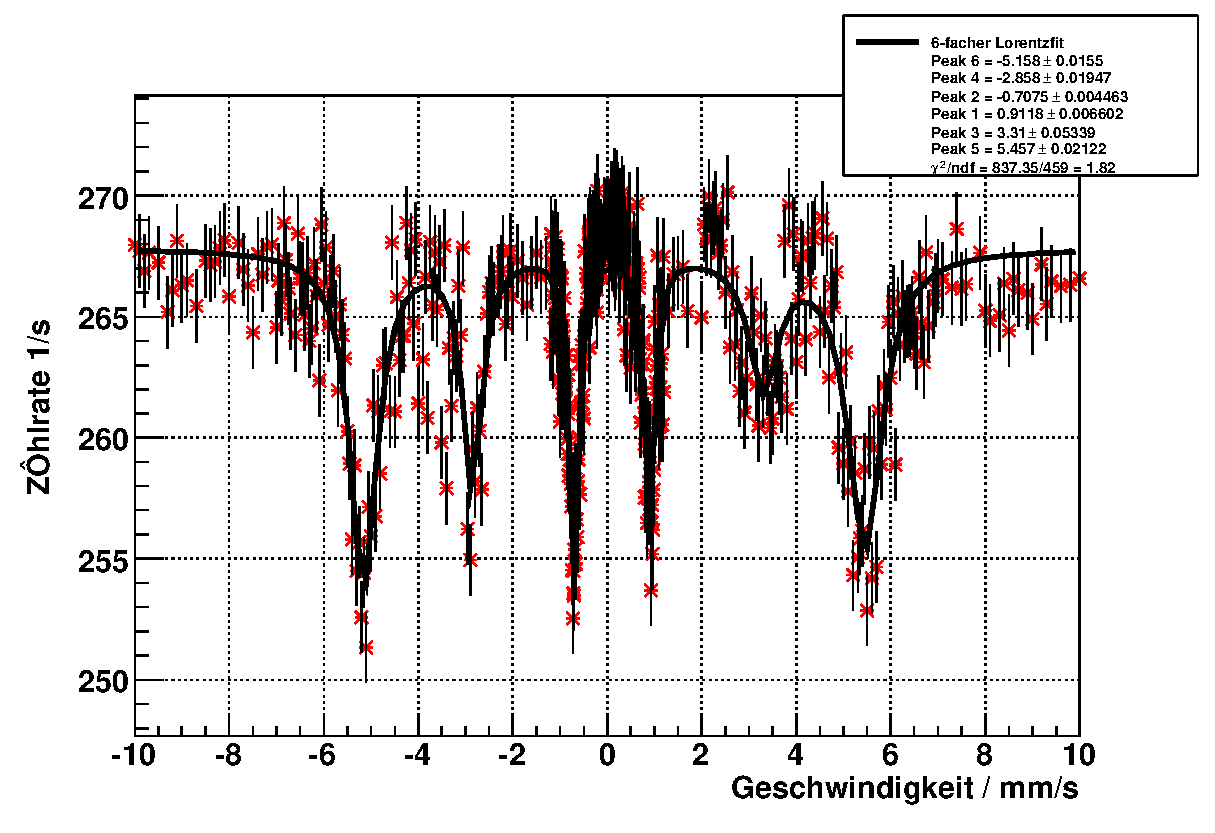
\includegraphics[width=0.9\linewidth]{pictures/eisen.eps}
}
\frame{\frametitle{Kurvenverlauf}
\begin{block}{Identifikation der Peaks}
\begin{align*}
 v_i = v_{iso} - v_{hfs}^i \hspace{5pt} \textnormal{    mit } v_{hfs}^i = \frac{c}{E_0} E_{hfs}^i = \frac{c}{E_0} \left( \frac{\mu_a m_a^i}{I_a} - \frac{\mu_g m_g^i}{I_g} \right) B
\label{geschw}
\end{align*}
\end{block}
\vfill
\begin{itemize}
 \item Mit Auswahlregel für Dipolstrahlung ($\Delta m = 0, \pm 1$) $\Rightarrow$ 6 mögliche Übergänge
 \item Je 2 Geschwindigkeiten unterscheiden sich nur durch Vorzeichen
\end{itemize}

}
\frame{\frametitle{Messdaten}
\begin{tabular}{|l|l|l|l|l|l|l|}
\hline
Peak& $\mu_a^i$ & $\mu_g^i$ & $v_{hfs}^i$ & $v_{mes}^i/\frac{mm}{s}$ & $E_{mes}^i/10^{-7} eV$ & \% Fehler\\
\hline
1 & $+\frac{3}{2}$ & $+\frac{1}{2}$ & $v_{hfs}^1$ & -5.158 & -2.48 & 0.72\\
2 & $+\frac{1}{2}$ & $+\frac{1}{2}$ & $v_{hfs}^2$ & -2.858 & -1.37 & 0.63\\
3 & $-\frac{1}{2}$ & $+\frac{1}{2}$ & $v_{hfs}^3$ & -0.7075 & -0.34 & 1.61\\
4 & $+\frac{1}{2}$ & $-\frac{1}{2}$ & $v_{hfs}^4 = -v_{hfs}^3$ & 0.9118 & -0.44 & 0.68\\
5 & $-\frac{1}{2}$ & $-\frac{1}{2}$ & $v_{hfs}^5 = -v_{hfs}^2$ & 3.31 & 1.59 & 0.39\\
6 & $-\frac{3}{2}$ & $-\frac{1}{2}$ & $v_{hfs}^6 = -v_{hfs}^1$ & 5.457 & 2.62 & 0.3\\
\hline
\end{tabular}
}

\frame{\frametitle{Isomerieverschiebung}
\begin{block}{Isomerieverschiebung}
\begin{align*}
 v_{iso} = \frac{v_{mes}^1+v_{mes}^6}{2} =\frac{v_{mes}^2+v_{mes}^5}{2} =\frac{v_{mes}^3+v_{mes}^4}{2}
\end{align*}
Wir erhielten als Ergebnisse:
\begin{tabular}{|l|lll|}
\hline
Peaks & $v_{iso}/\frac{mm}{s}$ & $E_{iso}/10^{-9}eV$ & \% Fehler\\
\hline
1 und 6& $-0.1021 \pm 0.004$ & $-4.91 \pm 0.19$ & 3.9\\
2 und 5& $-0.2262 \pm 0.028$ & $-10.8 \pm 1.4$ & 12.56\\
3 und 4& $-0.1497 \pm 0.013$ & $-7.195 \pm 0.63$ & 8.78\\
\hline
\end{tabular}
\end{block}
\vfill
\begin{align*}
 \textnormal{gew. Mittel: } v_{iso} = (-0.1083\pm 0.0038)\frac{mm}{s} \quad \textnormal{Lit.:}  v_{iso,Lit} = -0,110 \frac{mm}{s}
\end{align*}
}

\frame{\frametitle{Kernmagnetisches Moment}
}
\subsection{Ergebnisse}
\section{Die Entdeckung der Langsamkeit}
\end{document}

